\documentclass[../Languages.tex]{subfiles}

\begin{document}
\usec{Lua}\label{sec:lua}

\cd{Lua} is a lightweight, multi-paradigm programming language designed
primaryily for embedded systems and clients. \cd{Lua} is cross-platform, since
the interpreter is written in \cd{C}, and had a relatively simple \cd{C} API.

\cd{Lua} was originally designed in 1993 as a languages for extending software
applications to meet the increasing demand for customization at the time. It
provided the basic facilities of most procedural programming languages, but
more complicated or domain-specific features were not included; rather, it
included mechanisms for extending the language, allowing programmers to
implement such features. As \cd{Lua} was intended to be a general embeddable
extension language, the designers of \cd{Lua} focused on improving its
speed,portability, extensibility, and ease-of-use in development.

\subsection{Influence}\label{sub:influence}

\begin{Figure}
  \centering
  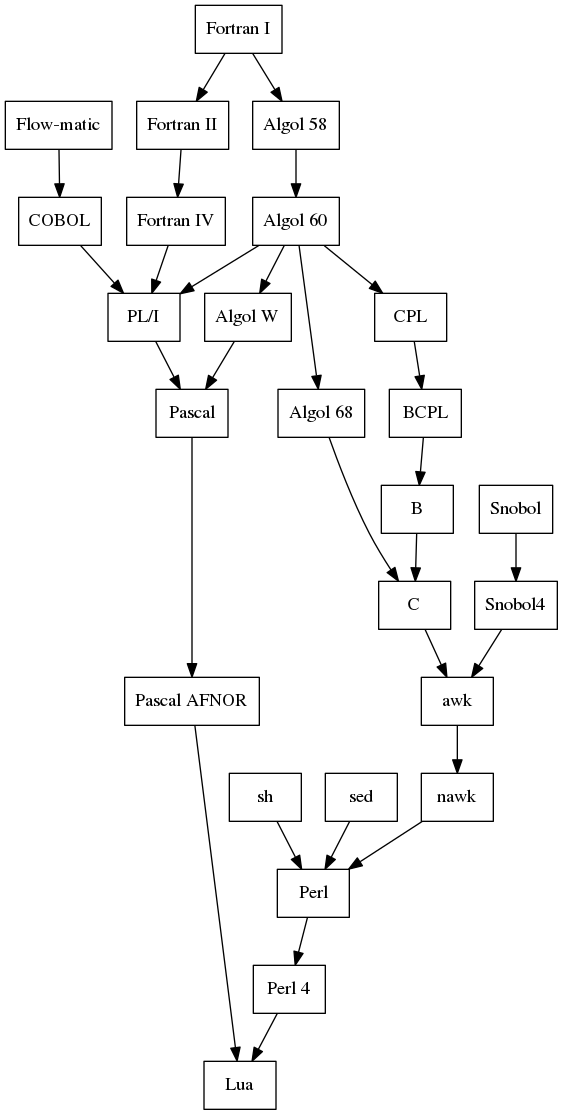
\includegraphics[height=0.5\textheight]{lua}
  \captionof{figure}{Inheritance diagram for \cd{Lua}.}
\end{Figure}

\newpage
\end{document}
